\documentclass[11pt,a4paper]{article}

% --- Paquetes básicos ---
\usepackage[utf8]{inputenc}
\usepackage[T1]{fontenc}
\usepackage[spanish,es-tabla]{babel}
\usepackage[margin=2.5cm]{geometry}
\usepackage{parskip}
\usepackage{setspace}
\onehalfspacing

% --- Matemáticas, figuras, tablas y código ---
\usepackage{amsmath,amssymb}
\usepackage{graphicx}
\usepackage{float}
\usepackage{booktabs}
\usepackage{xcolor}
\usepackage{listings}
\usepackage[hidelinks]{hyperref}

% --- Configuración sencilla para mostrar bloques de código Python ---
\definecolor{codebg}{RGB}{245,247,250}
\definecolor{codeblue}{RGB}{0,70,140}
\definecolor{codegreen}{RGB}{40,130,60}

\lstdefinestyle{pythonstyle}{
    language=Python,
    backgroundcolor=\color{codebg},
    frame=single,
    basicstyle=\ttfamily\footnotesize,
    keywordstyle=\color{codeblue}\bfseries,
    commentstyle=\color{codegreen}\itshape,
    breaklines=true,
    showstringspaces=false,
    numbers=left,
    numberstyle=\tiny\color{gray},
    literate={á}{{\'a}}1 {é}{{\'e}}1 {í}{{\'i}}1 {ó}{{\'o}}1 {ú}{{\'u}}1
             {ñ}{{\~n}}1 {º}{{\textordmasculine}}1 {°}{{$^\circ$}}1
}

% Busca las imágenes tanto en la raíz del proyecto como en la carpeta figuras/
\graphicspath{{./}{figuras/}{docs/figuras/}}

\begin{document}

% ==============================================================================
% PORTADA
% ==============================================================================
\begin{titlepage}
    \centering
    \vspace*{2cm}
    {\Large \textbf{UNIVERSITAT POLITÈCNICA DE VALÈNCIA}}\\[0.4cm]
    {\large Asignatura: \textit{Modelado y Control de Robots}}\\[2.5cm]

    \rule{\linewidth}{0.5mm}\\[0.4cm]
    {\LARGE \bfseries Modelado, Cinemática y Simulación de un Robot Manipulador de 3 GDL en MuJoCo}\\[0.2cm]
    \rule{\linewidth}{0.5mm}\\[2cm]

    {\large \textbf{Alumno:} Nacho \textit{(Escribe aquí tus apellidos)}}\\[0.4cm]
    {\large \textbf{Profesor:} J. Ernesto Solanes}\\[3cm]

    \vfill
    {\normalsize Curso 2025--2026}
\end{titlepage}

% ==============================================================================
% RESUMEN (SIN NUMERAR)
% ==============================================================================
\section*{Resumen}
\addcontentsline{toc}{section}{Resumen}

En este trabajo se ha diseñado, modelado y simulado desde cero un brazo robótico articulado de tres grados de libertad (configuración RRR) utilizando Python y el simulador físico MuJoCo. El diseño del robot está inspirado en una maqueta de escritorio formada por tres microservomotores comerciales tipo SG90: uno para el giro horizontal de la base, otro para levantar el hombro y un tercero para doblar el codo. Debido al tope físico de este tipo de servomotores de $180^\circ$ de recorrido total, cada articulación puede girar entre $-90^\circ$ y $+90^\circ$.

Para calcular el movimiento del robot se han aplicado paso a paso los métodos explicados en los apuntes de clase. La cinemática directa se ha resuelto mediante el algoritmo de Denavit-Hartenberg (DH), multiplicando las matrices de transformación de cada eslabón para hallar las coordenadas $(x, y, z)$ de la punta del brazo. Por su parte, la cinemática inversa se ha resuelto mediante el método geométrico, proyectando el robot sobre el plano del suelo y sobre el plano vertical para despejar los tres ángulos articulares con trigonometría básica y contemplando las dos posturas posibles del codo (\textit{codo abajo} o \texttt{down} y \textit{codo arriba} o \texttt{up}). Finalmente, se ha creado un panel de control en Tkinter conectado en tiempo real con el visor 3D de MuJoCo, comprobando que las posiciones calculadas por nuestras ecuaciones coinciden exactamente con las del simulador.

\newpage
\tableofcontents
\newpage

% ==============================================================================
% 1 INTRODUCCIÓN
% ==============================================================================
\section{Introducción}

\subsection{Contexto y justificación}
En robótica, antes de poder mover un brazo articulado para hacer cualquier tarea, necesitamos resolver dos preguntas fundamentales: saber dónde está la punta del robot cuando conocemos los ángulos de sus motores (cinemática directa) y saber qué ángulos debemos poner en los motores para llevar la punta a una coordenada concreta del espacio (cinemática inversa). Cuando no disponemos de un brazo físico en el laboratorio, utilizar un simulador físico como MuJoCo es una alternativa ideal, ya que nos permite construir el robot en el ordenador y poner a prueba nuestras fórmulas matemáticas viendo cómo se mueve en 3D bajo el efecto de la gravedad y con límites reales en sus articulaciones.

Este proyecto se ha desarrollado para la asignatura \textit{Modelado y Control de Robots}. Su objetivo principal es aplicar de forma práctica las ecuaciones del tema de cinemática vistas en clase, programándolas nosotros mismos en Python de manera sencilla y transparente, sin depender de librerías externas que hagan los cálculos de forma oculta.

\subsection{Objetivos}
El objetivo general del trabajo es modelar un robot manipulador de 3 grados de libertad en MuJoCo y controlarlo mediante cinemática directa e inversa desde una interfaz gráfica propia. Los objetivos específicos son:
\begin{enumerate}
    \item Construir el modelo 3D del robot en un archivo XML de MuJoCo (\texttt{robot.xml}) con tres articulaciones rotacionales, colores diferenciados por eslabón y límites de $[-90^\circ, +90^\circ]$.
    \item Plantear y programar la cinemática directa del robot aplicando el método de Denavit-Hartenberg de los apuntes de la asignatura.
    \item Plantear y programar la cinemática inversa mediante el método geométrico de clase, permitiendo elegir entre las dos configuraciones de codo (\texttt{down} y \texttt{up}) y avisando cuando un punto sea inalcanzable.
    \item Crear una interfaz gráfica intuitiva que permita mover el robot tanto por ángulos como por coordenadas $(X, Y, Z)$, mostrando en el visor 3D los ejes del robot y el punto objetivo.
\end{enumerate}

% ==============================================================================
% 2 MARCO TEÓRICO
% ==============================================================================
\section{Marco Teórico}

\subsection{Conceptos principales}
Un robot manipulador se compone de barras rígidas llamadas \textit{eslabones} conectadas por \textit{articulaciones} que producen el movimiento. Como nuestro brazo tiene 3 articulaciones de giro (tipo RRR), su postura en cualquier instante queda definida por tres ángulos: $q = [\theta_1, \theta_2, \theta_3]^T$.

\textbf{Cinemática Directa (Método de Denavit-Hartenberg):}
Sirve para calcular en qué coordenadas $(x, y, z)$ está la punta del robot a partir de los tres ángulos $(\theta_1, \theta_2, \theta_3)$. El método de Denavit-Hartenberg explicado en los apuntes de clase coloca un sistema de ejes $(X, Y, Z)$ en cada articulación y resume la forma de cada eslabón con solo 4 parámetros $(d_i, \theta_i, a_i, \alpha_i)$:
\begin{itemize}
    \item $d_i$: altura o desplazamiento a lo largo del eje $z_{i-1}$.
    \item $\theta_i$: ángulo de giro del motor alrededor del eje $z_{i-1}$.
    \item $a_i$: longitud del eslabón medida a lo largo del eje $x_i$.
    \item $\alpha_i$: giro de inclinación entre el eje $z_{i-1}$ de un motor y el eje $z_i$ del siguiente.
\end{itemize}

Con estos 4 datos se rellena la matriz de transformación $A_i$ de cada eslabón:
\begin{equation}
    A_i = \text{Rot}_{z,\theta_i} \cdot \text{Trans}_{z,d_i} \cdot \text{Trans}_{x,a_i} \cdot \text{Rot}_{x,\alpha_i} =
    \begin{bmatrix}
        \cos\theta_i & -\sin\theta_i\cos\alpha_i & \sin\theta_i\sin\alpha_i & a_i\cos\theta_i \\
        \sin\theta_i & \cos\theta_i\cos\alpha_i & -\cos\theta_i\sin\alpha_i & a_i\sin\theta_i \\
        0 & \sin\alpha_i & \cos\alpha_i & d_i \\
        0 & 0 & 0 & 1
    \end{bmatrix}
    \label{eq:dh_general}
\end{equation}
Multiplicando las matrices de los tres eslabones ($T_3^0 = A_1 \cdot A_2 \cdot A_3$), los tres primeros números de la última columna nos dan directamente la posición $(x_c, y_c, z_c)$ de la punta respecto a la base.

\textbf{Cinemática Inversa (Método Geométrico):}
Resuelve el paso inverso: si queremos llevar la punta del robot a unas coordenadas concretas $(x_c, y_c, z_c)$, calcula qué ángulos $(\theta_1, \theta_2, \theta_3)$ hay que mandar a los motores. En lugar de despejar matrices complicadas, el método geométrico de los apuntes dibuja el triángulo que forman el brazo y el antebrazo y utiliza el teorema del coseno y la función arcotangente de dos argumentos $\text{atan2}(y, x)$ para sacar los tres ángulos de forma directa.

\subsection{Tecnologías o herramientas}
Para desarrollar el trabajo se han elegido las siguientes herramientas en Windows:
\begin{itemize}
    \item \textbf{MuJoCo frente a otros motores como Unity:} Aunque existía la opción de usar Unity, se ha elegido MuJoCo porque está diseñado específicamente para robótica y utiliza el mismo sistema de coordenadas de mano derecha con el eje $Z$ vertical hacia arriba que usamos en los apuntes de clase (mientras que Unity es un motor de videojuegos que usa mano izquierda con el eje $Y$ hacia arriba, lo que obligaría a cambiar signos y ejes respecto a la teoría).
    \item \textbf{Modelado mediante archivo XML (MJCF):} En MuJoCo los robots no se dibujan con el ratón, sino escribiendo un archivo de texto XML (\texttt{model/robot.xml}) donde cada eslabón (\texttt{<body>}) se mete dentro del eslabón anterior como si fueran muñecas rusas. Así, cuando gira la base, arrastra automáticamente al hombro, al codo y a la punta.
    \item \textbf{Python 3.13, NumPy y Tkinter:} Con Python y NumPy programamos las multiplicaciones de matrices de forma muy limpia en pocas líneas, y con Tkinter hemos creado la ventana de control con deslizadores y botones conectada al visor 3D.
\end{itemize}

% ==============================================================================
% 3 METODOLOGÍA
% ==============================================================================
\section{Metodología}

Para llevar a cabo el desarrollo y la validación del robot de forma ordenada, la metodología del trabajo se divide en las siguientes tres etapas:

\begin{enumerate}
    \item \textbf{Construcción del modelo 3D en MuJoCo y prueba de movimiento articular.} Consiste en definir la geometría del brazo, sus articulaciones y sus posiciones de referencia en el archivo \texttt{robot.xml}, programar el control básico en \texttt{robot\_control.py} y comprobar cómo se mueven los eslabones al cambiar los ángulos.
    \item \textbf{Cálculo de la Cinemática Directa por Denavit-Hartenberg y comprobación frente a MuJoCo.} Consiste en obtener la tabla de parámetros DH del robot, programar el cálculo de la matriz $T_3^0$ en \texttt{kinematics.py} y verificar en 9 posturas distintas que la posición $(x, y, z)$ calculada por nuestras ecuaciones coincide con la que mide el simulador, además de dibujar su espacio de trabajo.
    \item \textbf{Cálculo de la Cinemática Inversa geométrica, configuraciones de codo e interfaz gráfica.} Consiste en programar las ecuaciones geométricas para calcular $(\theta_1, \theta_2, \theta_3)$ a partir de un punto objetivo $(X, Y, Z)$, comparar las dos soluciones de codo (\texttt{down} y \texttt{up}), comprobar el aviso de error ante puntos fuera de alcance y validar todo el conjunto desde la interfaz gráfica (\texttt{gui.py}).
\end{enumerate}

% ------------------------------------------------------------------------------
\subsection{Construcción del modelo 3D en MuJoCo y prueba de movimiento articular}
En esta primera parte se ha construido el robot dentro del archivo \texttt{model/robot.xml} usando cilindros, cápsulas y esferas con medidas en metros y colores distintos para distinguir cada parte a simple vista:
\begin{itemize}
    \item \textbf{Base fija (gris oscuro) y Articulación 1 ($J_1$, giro de base):} La base está fija en el suelo $(0,0,0)$. A una altura de $d_1 = 0.060\text{ m}$ ($6\text{ cm}$) se coloca la torreta blanca con la primera bisagra (\texttt{joint\_base\_yaw}), que gira en horizontal alrededor del eje vertical $Z$ (\texttt{axis="0 0 1"}).
    \item \textbf{Brazo superior (naranja) y Articulación 2 ($J_2$, hombro):} Nace también a $0.060\text{ m}$ de altura. Su bisagra (\texttt{joint\_shoulder\_pitch}) gira en vertical (\texttt{axis="0 -1 0"}) para que los ángulos positivos levanten el brazo hacia arriba. El tubo naranja mide exactamente $a_2 = 0.100\text{ m}$ ($10\text{ cm}$).
    \item \textbf{Antebrazo (verde), Articulación 3 ($J_3$, codo) y Punta (bola roja):} Al final del brazo naranja se sitúa el codo (\texttt{joint\_elbow\_pitch}). El tubo verde mide $0.080\text{ m}$ y termina en una bola roja a $0.020\text{ m}$ donde ponemos el sensor de posición (\texttt{site\_end\_effector}), sumando una longitud total desde el codo hasta la punta de $a_3 = 0.080 + 0.020 = 0.100\text{ m}$ ($10\text{ cm}$).
    \item \textbf{Marcador visual del objetivo (bola verde semitransparente):} Además del robot, se ha añadido en el visor 3D una esfera verde flotante (\texttt{target\_marker}) que indica visualmente en qué coordenada $(X, Y, Z)$ queremos colocar la punta. Cuando el robot alcanza su objetivo, la bola roja de la punta se mete exactamente dentro de la bola verde.
\end{itemize}

\textbf{¿Por qué los límites son de $-90^\circ$ a $+90^\circ$ ($180^\circ$ en total)?}
Porque el diseño imita a los microservos reales SG90 (representados como cajitas azules en las articulaciones). Estos servos tienen un tope mecánico interno que solo les permite girar $180^\circ$: desde $-90^\circ$ hacia un lado hasta $+90^\circ$ hacia el otro pasando por el centro ($0^\circ$).

\textbf{Posición Origen $[0^\circ, 0^\circ, 0^\circ]$ frente a Posición Home (postura de codo):}
En la teoría de Denavit-Hartenberg (igual que ocurre en robots industriales como el UR3), cuando los tres ángulos valen cero ($[0^\circ, 0^\circ, 0^\circ]$), el brazo queda totalmente plano y estirado a lo largo del eje $X$. Como visualmente es mucho más intuitivo ver el robot levantado con forma de brazo, hemos configurado dos botones rápidos en la interfaz: la \textbf{Posición Origen} ($[0^\circ, 0^\circ, 0^\circ]$, estirado) y la \textbf{Posición Home} ($[0^\circ, +45^\circ, -30^\circ]$, con el hombro levantado y el codo flexionado, que es la postura en la que arranca el programa).

% ------------------------------------------------------------------------------
\subsection{Cálculo de la Cinemática Directa por Denavit-Hartenberg y comprobación frente a MuJoCo}
En esta segunda parte se obtienen las ecuaciones de la Cinemática Directa aplicando la tabla de Denavit-Hartenberg explicada en clase sobre los 3 sistemas de ejes del robot (que se pueden ver directamente en el visor 3D activando la casilla \textit{«Mostrar sistemas XYZ»}):
\begin{itemize}
    \item El eslabón 1 sube $d_1 = 0.060\text{ m}$ desde el suelo hasta el hombro y gira $\alpha_1 = +\pi/2$ ($90^\circ$) porque el eje de la base es vertical y el eje del hombro es horizontal.
    \item Los eslabones 2 (brazo naranja) y 3 (antebrazo verde + punta roja) se mueven en el mismo plano vertical, por lo que no tienen desplazamiento lateral ($d_2 = d_3 = 0$) ni torsión entre sus ejes ($\alpha_2 = \alpha_3 = 0$), y sus longitudes son $a_2 = 0.100\text{ m}$ y $a_3 = 0.100\text{ m}$.
\end{itemize}

\begin{table}[H]
    \centering
    \caption{Tabla de parámetros de Denavit-Hartenberg (DH) de nuestro robot.}
    \label{tab:dh}
    \begin{tabular}{ccccc}
        \toprule
        \textbf{Eslabón $i$} & \textbf{$d_i$ (m)} & \textbf{$\theta_i$ (rad)} & \textbf{$a_i$ (m)} & \textbf{$\alpha_i$ (rad)} \\
        \midrule
        1 (Base -- Hombro) & $d_1 = 0.060$ & $\theta_1$ & $0$ & $+\pi/2$ \\
        2 (Brazo naranja) & $0$ & $\theta_2$ & $a_2 = 0.100$ & $0$ \\
        3 (Antebrazo verde + Punta) & $0$ & $\theta_3$ & $a_3 = 0.100$ & $0$ \\
        \bottomrule
    \end{tabular}
\end{table}

Sustituyendo cada fila de la Tabla~\ref{tab:dh} en la matriz general de la Ecuación~\eqref{eq:dh_general}, obtenemos las tres matrices individuales $A_1, A_2$ y $A_3$:
\begin{equation}
    A_1 =
    \begin{bmatrix}
        \cos\theta_1 & 0 & \sin\theta_1 & 0 \\
        \sin\theta_1 & 0 & -\cos\theta_1 & 0 \\
        0 & 1 & 0 & d_1 \\
        0 & 0 & 0 & 1
    \end{bmatrix}, \quad
    A_2 =
    \begin{bmatrix}
        \cos\theta_2 & -\sin\theta_2 & 0 & a_2\cos\theta_2 \\
        \sin\theta_2 & \cos\theta_2 & 0 & a_2\sin\theta_2 \\
        0 & 0 & 1 & 0 \\
        0 & 0 & 0 & 1
    \end{bmatrix}, \quad
    A_3 =
    \begin{bmatrix}
        \cos\theta_3 & -\sin\theta_3 & 0 & a_3\cos\theta_3 \\
        \sin\theta_3 & \cos\theta_3 & 0 & a_3\sin\theta_3 \\
        0 & 0 & 1 & 0 \\
        0 & 0 & 0 & 1
    \end{bmatrix}
\end{equation}

Al multiplicar las tres matrices ($T_3^0 = A_1 \cdot A_2 \cdot A_3$), la última columna nos da las fórmulas de las coordenadas $(x_c, y_c, z_c)$ de la bola roja de la punta:
\begin{align}
    x_c &= \cos\theta_1 \left( a_2\cos\theta_2 + a_3\cos(\theta_2 + \theta_3) \right) \label{eq:cd_x} \\
    y_c &= \sin\theta_1 \left( a_2\cos\theta_2 + a_3\cos(\theta_2 + \theta_3) \right) \label{eq:cd_y} \\
    z_c &= d_1 + a_2\sin\theta_2 + a_3\sin(\theta_2 + \theta_3) \label{eq:cd_z}
\end{align}

En \texttt{src/kinematics.py} se ha programado esta multiplicación de matrices tal como se ve en el Listado~\ref{lst:cd}.

\begin{lstlisting}[style=pythonstyle, caption={Cálculo de la Cinemática Directa por Denavit-Hartenberg en \texttt{src/kinematics.py}.}, label={lst:cd}]
def dh_matrix(d_i: float, theta_i: float, a_i: float, alpha_i: float) -> np.ndarray:
    ct, st = float(np.cos(theta_i)), float(np.sin(theta_i))
    ca, sa = float(np.cos(alpha_i)), float(np.sin(alpha_i))
    return np.array([
        [ct, -st * ca,  st * sa, a_i * ct],
        [st,  ct * ca, -ct * sa, a_i * st],
        [0.0,      sa,       ca,      d_i],
        [0.0,     0.0,      0.0,      1.0],
    ], dtype=float)

def forward_kinematics_deg(angles_deg: Sequence[float]) -> np.ndarray:
    q_rad = np.deg2rad(np.asarray(angles_deg, dtype=float))
    dh_rows = get_dh_table_rad(q_rad)
    T_0_3 = dh_matrix(*dh_rows[0]) @ dh_matrix(*dh_rows[1]) @ dh_matrix(*dh_rows[2])
    return T_0_3[:3, 3].copy()
\end{lstlisting}

% ------------------------------------------------------------------------------
\subsection{Cálculo de la Cinemática Inversa geométrica, configuraciones de codo e interfaz gráfica}
En esta tercera parte se resuelve la Cinemática Inversa siguiendo el método geométrico de los apuntes de la asignatura. Si el usuario escribe unas coordenadas objetivo $(x_c, y_c, z_c)$:

\begin{enumerate}
    \item \textbf{Ángulo de la base ($\theta_1$):} Mirando el robot desde arriba (plano $x_0 - y_0$), el ángulo que debe girar la base para apuntar hacia el objetivo es:
    \begin{equation}
        \theta_1 = \text{atan2}(y_c, x_c)
        \label{eq:ci_theta1}
    \end{equation}
    \item \textbf{Ángulo del codo ($\theta_3$):} Mirando el brazo de perfil (plano vertical $z_0 - r$), la distancia horizontal al objetivo es $r = \sqrt{x_c^2 + y_c^2}$ y la altura desde el hombro es $s = z_c - d_1$. Por el teorema del coseno en el triángulo que forman el brazo ($a_2$) y el antebrazo ($a_3$), calculamos $D = \cos\theta_3$:
    \begin{equation}
        D = \frac{x_c^2 + y_c^2 + (z_c - d_1)^2 - a_2^2 - a_3^2}{2\, a_2\, a_3}
        \label{eq:ci_D}
    \end{equation}
    Como el coseno de un ángulo nunca puede ser mayor que $1$ ni menor que $-1$, si sale $|D| > 1$ significa que el punto está demasiado lejos (a más de $0.200\text{ m}$ del hombro) y el programa avisa de que es inalcanzable. Si $|D| \le 1$, hallamos $\sin\theta_3$ y el ángulo $\theta_3$:
    \begin{equation}
        \sin\theta_3 = \pm\sqrt{1 - D^2}, \qquad \theta_3 = \text{atan2}(\sin\theta_3, \cos\theta_3)
        \label{eq:ci_theta3}
    \end{equation}
    El signo $\pm$ nos permite elegir entre las dos posturas posibles del codo para llegar al mismo sitio: la configuración \texttt{down} ($\theta_3 \le 0^\circ$, hombro alto y codo flexionado hacia abajo) y la configuración \texttt{up} ($\theta_3 \ge 0^\circ$, hombro bajo y codo flexionado hacia arriba).
    \item \textbf{Ángulo del hombro ($\theta_2$):} Una vez sabido $\theta_3$, calculamos el ángulo interno $\beta$ del triángulo y se lo restamos a la inclinación general:
    \begin{equation}
        \beta = \text{atan2}\left(a_3\sin\theta_3,\, a_2 + a_3\cos\theta_3\right), \qquad \theta_2 = \text{atan2}(s, r) - \beta
        \label{eq:ci_theta2}
    \end{equation}
    \textit{(Nota práctica: en un par de diapositivas de los apuntes se escribe la notación $\text{atan2}(\cos, \sin)$, pero en Python la función \texttt{np.arctan2(y, x)} pide siempre primero el seno y luego el coseno)}.
\end{enumerate}

\begin{lstlisting}[style=pythonstyle, caption={Cálculo de la Cinemática Inversa geométrica en \texttt{src/kinematics.py}.}, label={lst:ci}]
r_sq = xc**2 + yc**2
r = float(np.sqrt(r_sq))
s = zc - d1
D = (r_sq + s**2 - a2**2 - a3**2) / (2.0 * a2 * a3)
if abs(D) > 1.0 + tol:
    raise ValueError("Objetivo fuera del espacio de trabajo (|D| > 1).")

sin_theta3 = sign_e * np.sqrt(max(0.0, 1.0 - D**2))
cos_theta3 = D
theta3_rad = float(np.arctan2(sin_theta3, cos_theta3))
beta = float(np.arctan2(a3 * sin_theta3, a2 + a3 * cos_theta3))
theta2_rad = float(np.arctan2(s, r_proj) - beta)
\end{lstlisting}

Por último, el programa comprueba que los tres ángulos $[\theta_1, \theta_2, \theta_3]$ estén dentro de $[-90^\circ, +90^\circ]$ antes de mover el robot.

% ==============================================================================
% 4 RESULTADOS OBTENIDOS
% ==============================================================================
\section{Resultados obtenidos}

Siguiendo exactamente el mismo orden de los tres puntos explicados en la Metodología, a continuación se desarrollan y analizan los resultados obtenidos en cada uno de ellos.

% ------------------------------------------------------------------------------
\subsection{Construcción del modelo 3D en MuJoCo y prueba de movimiento articular}
Al ejecutar \texttt{python main.py}, el simulador arranca con el robot en su posición inicial (\textit{Home}) con ángulos $[0^\circ, +45^\circ, -30^\circ]$, situando la punta en $[0.1673, 0.0000, 0.1566]\text{ m}$ (Figura~\ref{fig:cap_manual_1}). Desde el panel de control es posible activar en tiempo real los ejes de giro ($J_1, J_2, J_3$) y los sistemas de coordenadas locales ($XYZ$) de cada articulación.

\begin{figure}[H]
    \centering
    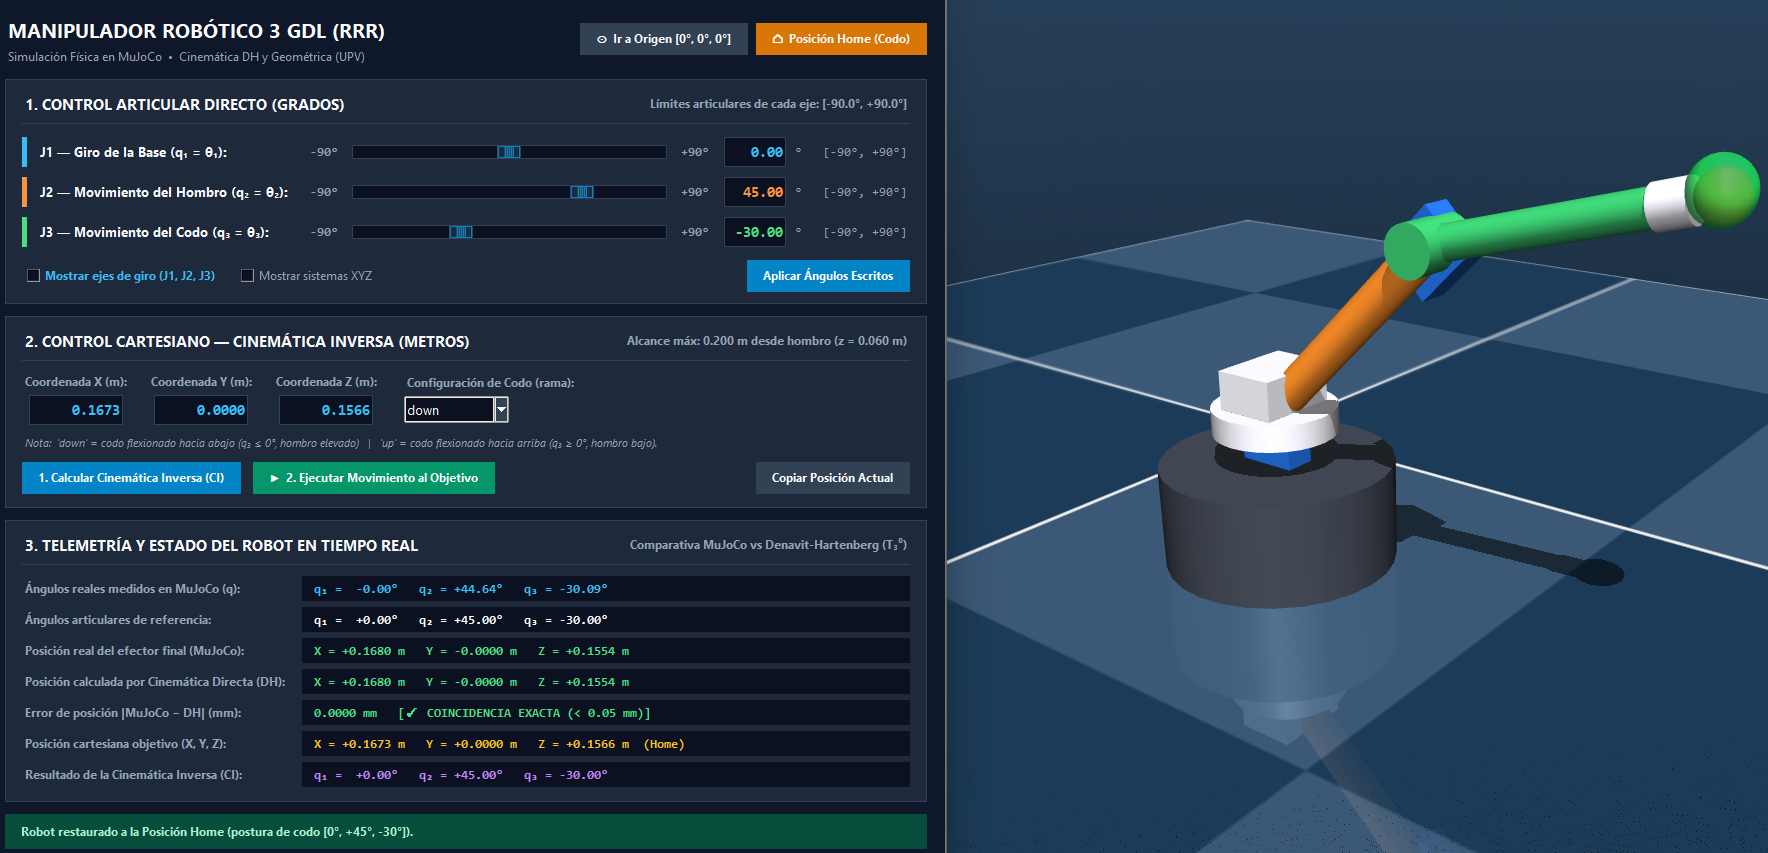
\includegraphics[width=0.95\textwidth]{captura_interfaz.png}
    \caption{Interfaz gráfica y visor 3D de MuJoCo mostrando el robot en su posición inicial (\textit{Home}).}
    \label{fig:cap_manual_1}
\end{figure}

Para comprobar cómo responden los tres motores del robot, se realizó una prueba partiendo de $[0^\circ, 0^\circ, 0^\circ]$ y moviendo un motor cada segundo: primero la base $J_1$ a $+45^\circ$ (en $t = 0.5\text{ s}$), luego el hombro $J_2$ a $+45^\circ$ (en $t = 1.5\text{ s}$) y por último el codo $J_3$ a $-30^\circ$ (en $t = 2.5\text{ s}$), tal y como se muestra en la Figura~\ref{fig:res_proc1}. De esta prueba se extraen dos conclusiones principales:
\begin{itemize}
    \item \textbf{Respuesta suave y rápida:} En cada gráfica se ve cómo el ángulo real de MuJoCo (línea continua de color) sube o baja suavemente hasta alcanzar el ángulo ordenado (línea discontinua) en unos $0.35\text{ s}$, sin pasarse de largo ni rebotar.
    \item \textbf{Protección de límites mecánicos:} Si se introduce un ángulo fuera del rango permitido de $[-90^\circ, +90^\circ]$ (por ejemplo, $130^\circ$), el sistema lo recorta automáticamente al límite del servo SG90 ($+90^\circ$) y muestra un aviso en la interfaz.
\end{itemize}

\begin{figure}[H]
    \centering
    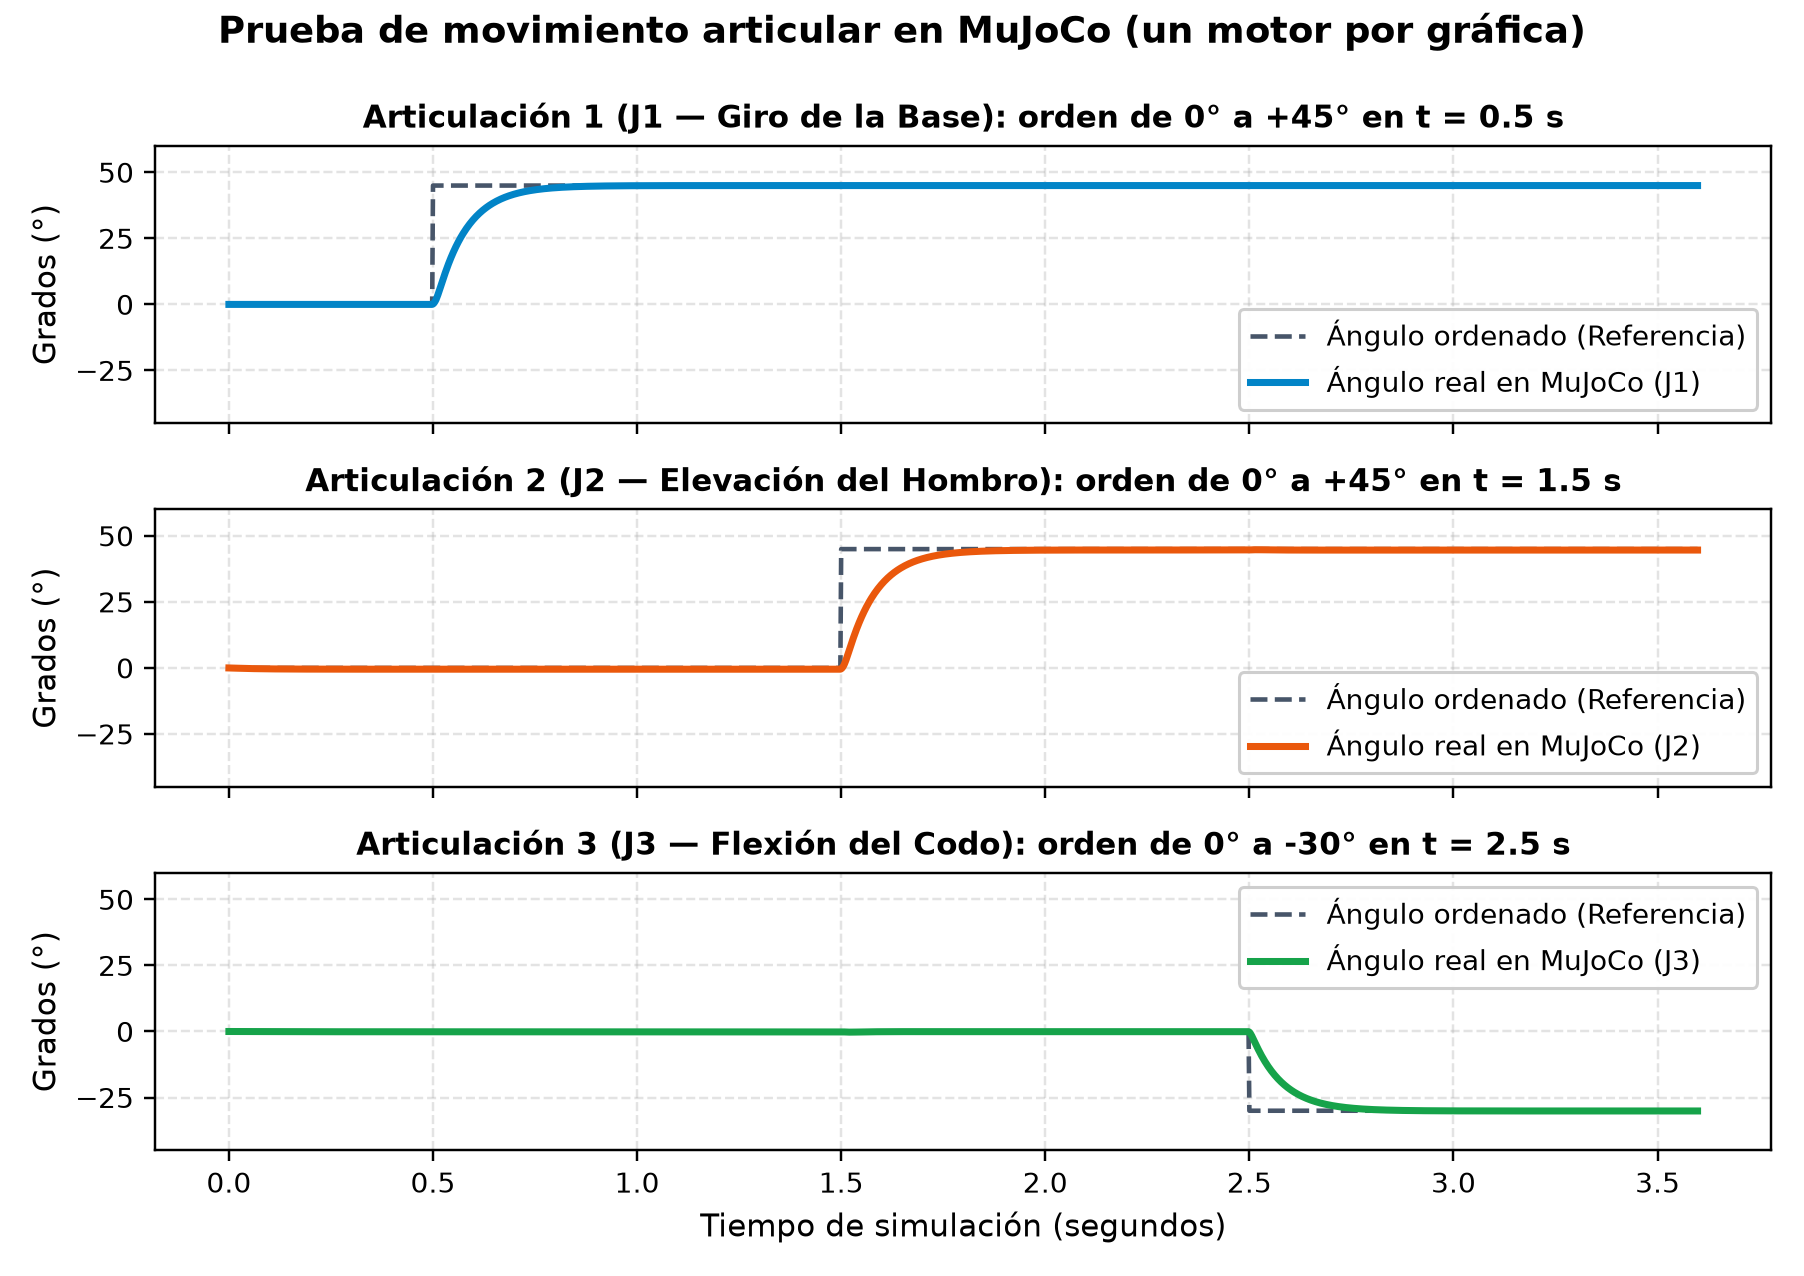
\includegraphics[width=0.95\textwidth]{fig_control_motores.png}
    \caption{Prueba de movimiento articular en MuJoCo: cada gráfica muestra cómo un motor ($J_1$ azul, $J_2$ naranja, $J_3$ verde) alcanza el ángulo que le pedimos (línea discontinua).}
    \label{fig:res_proc1}
\end{figure}

% ------------------------------------------------------------------------------
\subsection{Cálculo de la Cinemática Directa por Denavit-Hartenberg y comprobación frente a MuJoCo}
En la Cinemática Directa sabemos cuánto ha girado cada motor y queremos saber en qué coordenada $(X, Y, Z)$ queda la punta del robot: cada articulación es una matriz de $4 \times 4$, multiplicamos las tres ($T_3^0 = A_1 \cdot A_2 \cdot A_3$) y la última columna nos da directamente una única respuesta con la posición de la punta.

Para comprobarlo de forma sencilla en el simulador, se han probado 4 posturas fáciles de ver a simple vista, comparando el resultado de nuestra fórmula con la medida de MuJoCo (Tabla~\ref{tab:res_dh}):

\begin{enumerate}
    \item \textbf{Postura Origen $[0^\circ, 0^\circ, 0^\circ]$:} Con el brazo totalmente estirado hacia delante, la punta queda a $X = 0.10 + 0.10 = 0.2000\text{ m}$ y a la altura del hombro $Z = 0.0600\text{ m}$.
    \item \textbf{Postura Home $[0^\circ, +45^\circ, -30^\circ]$:} La postura inicial con el hombro levantado y el codo doblado, que sitúa la punta en $[0.1673, 0.0000, 0.1566]\text{ m}$.
    \item \textbf{Postura Vertical $[0^\circ, +90^\circ, 0^\circ]$:} Levantando el hombro $+90^\circ$ hacia el techo, la punta alcanza la altura máxima del robot: $Z = 0.06\text{ (base)} + 0.10\text{ (brazo)} + 0.10\text{ (antebrazo)} = 0.2600\text{ m}$.
    \item \textbf{Giro lateral $[+90^\circ, 0^\circ, 0^\circ]$:} Girando la base $+90^\circ$ hacia la izquierda con el brazo estirado, los $0.2000\text{ m}$ pasan del eje $X$ al eje $Y$.
\end{enumerate}

\begin{table}[H]
    \centering
    \caption{Comprobación de la Cinemática Directa (Denavit-Hartenberg) frente a MuJoCo en 4 posturas clave.}
    \label{tab:res_dh}
    \small
    \begin{tabular}{llccc}
        \toprule
        \textbf{Postura} & \textbf{Ángulos $[\theta_1, \theta_2, \theta_3]$} & \textbf{Cálculo DH $[x_c, y_c, z_c]$ (m)} & \textbf{Medida MuJoCo $[x, y, z]$ (m)} & \textbf{Error (mm)} \\
        \midrule
        1. Origen (estirado) & $[0^\circ,\, 0^\circ,\, 0^\circ]$ & $[+0.2000,\, +0.0000,\, +0.0600]$ & $[+0.2000,\, +0.0000,\, +0.0600]$ & $0.0000$ \\
        2. Home (codo) & $[0^\circ,\, +45^\circ,\, -30^\circ]$ & $[+0.1673,\, +0.0000,\, +0.1566]$ & $[+0.1673,\, +0.0000,\, +0.1566]$ & $0.0000$ \\
        3. Vertical (arriba) & $[0^\circ,\, +90^\circ,\, 0^\circ]$ & $[+0.0000,\, +0.0000,\, +0.2600]$ & $[+0.0000,\, +0.0000,\, +0.2600]$ & $0.0000$ \\
        4. Giro Base $+90^\circ$ & $[+90^\circ,\, 0^\circ,\, 0^\circ]$ & $[+0.0000,\, +0.2000,\, +0.0600]$ & $[+0.0000,\, +0.2000,\, +0.0600]$ & $0.0000$ \\
        \bottomrule
    \end{tabular}
\end{table}

Como muestra la Tabla~\ref{tab:res_dh}, el cálculo matemático y el simulador coinciden con $0.0000\text{ mm}$ de diferencia. Además, en la Figura~\ref{fig:res_proc2} (\texttt{fig\_espacio\_trabajo.png}) se muestra el robot visto de perfil en esas tres primeras posturas sobre la nube azul de su \textbf{espacio de trabajo}, que representa todos los puntos a los que puede llegar la punta moviendo los motores entre $-90^\circ$ y $+90^\circ$.

\begin{figure}[H]
    \centering
    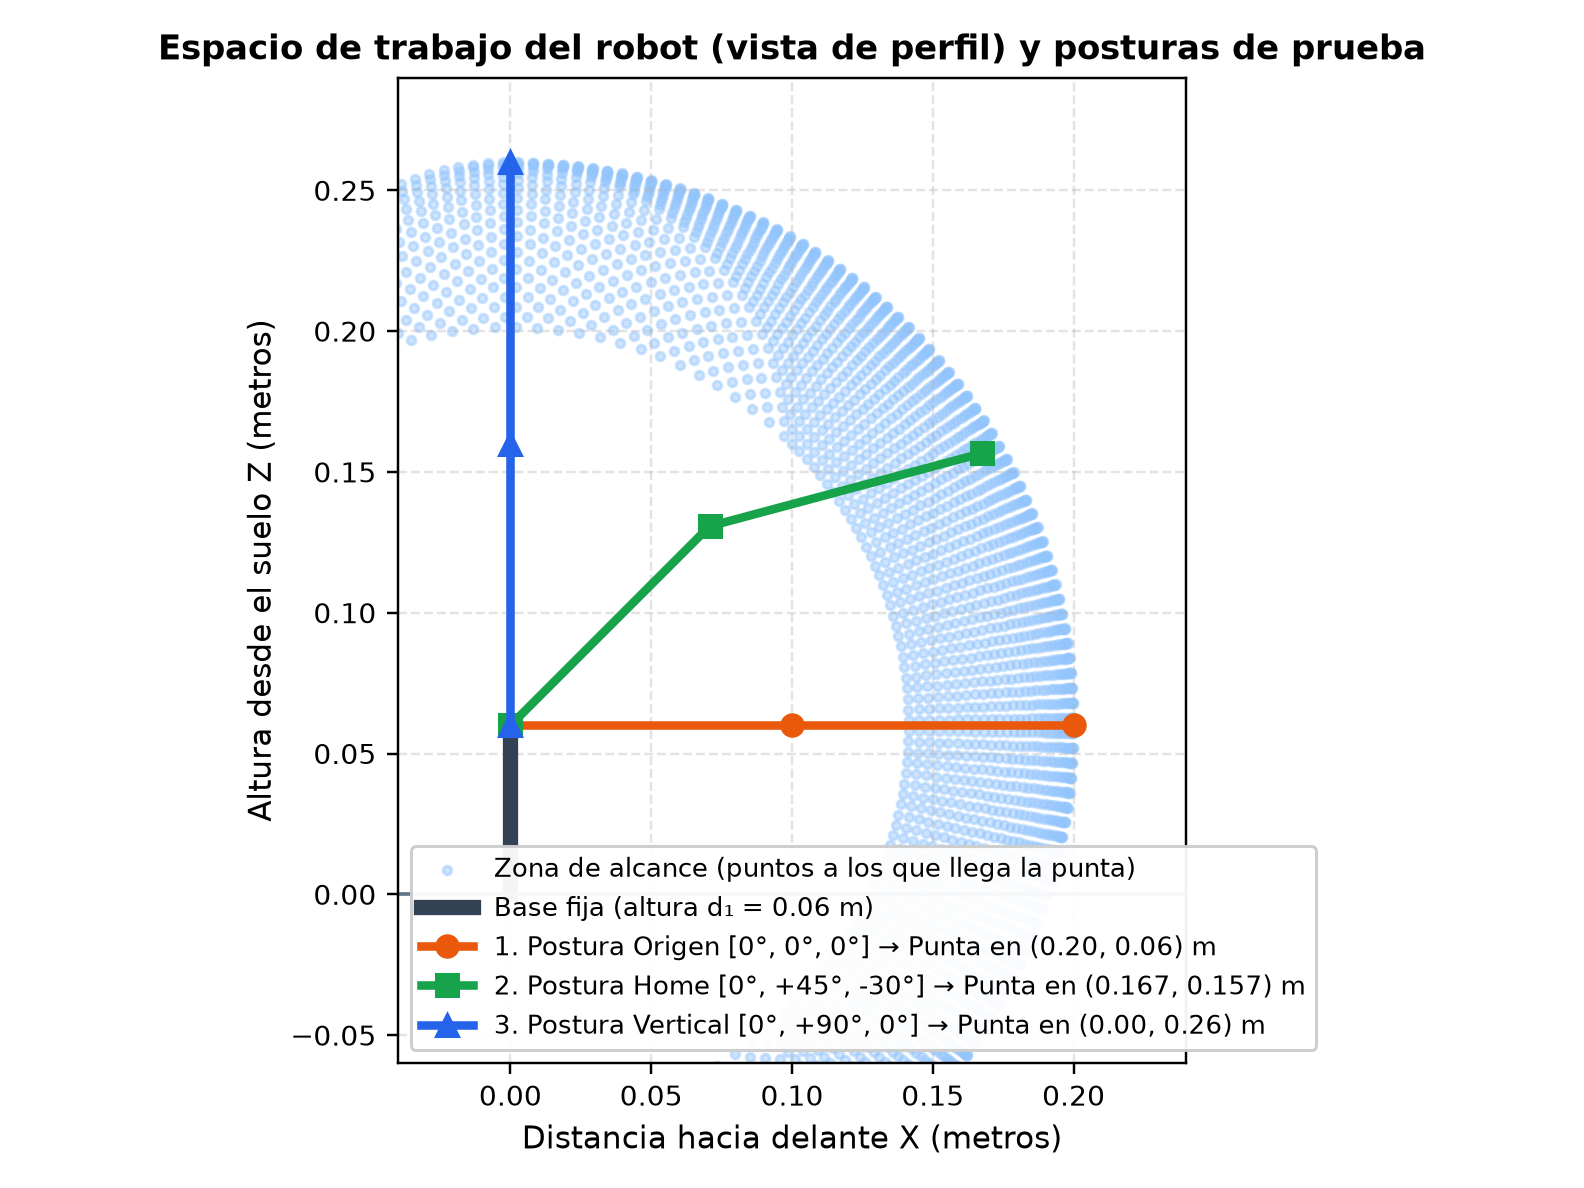
\includegraphics[width=0.78\textwidth]{fig_espacio_trabajo.png}
    \caption{Vista de perfil del espacio de trabajo del robot (zona azul) mostrando las posturas Origen (naranja), Home (verde) y Vertical (azul).}
    \label{fig:res_proc2}
\end{figure}

% ------------------------------------------------------------------------------
\subsection{Cálculo de la Cinemática Inversa geométrica, configuraciones de codo e interfaz gráfica}
En la Cinemática Inversa hacemos lo contrario que en la directa: escribimos la coordenada $(X, Y, Z)$ a la que queremos llevar la punta (por ejemplo, $[0.14, 0.05, 0.12]\text{ m}$) y el programa calcula qué ángulos hay que poner en los tres motores.

Lo más interesante de esta prueba es que \textbf{existen dos posturas distintas} para llegar exactamente al mismo punto, según elijamos la opción de codo \texttt{down} o \texttt{up} (Tabla~\ref{tab:res_ci}).

\begin{table}[H]
    \centering
    \caption{Las dos soluciones de Cinemática Inversa para llegar al punto $[0.140, 0.050, 0.120]\text{ m}$.}
    \label{tab:res_ci}
    \begin{tabular}{lcccc}
        \toprule
        \textbf{Configuración de Codo} & \textbf{$\theta_1$ (°)} & \textbf{$\theta_2$ (°)} & \textbf{$\theta_3$ (°)} & \textbf{Coordenada alcanzada (m)} \\
        \midrule
        Rama \texttt{down} (hombro alto, codo abajo) & $+19.65^\circ$ & $+58.70^\circ$ & $-73.44^\circ$ & $[+0.1400,\, +0.0500,\, +0.1200]$ \\
        Rama \texttt{up} (hombro bajo, codo arriba) & $+19.65^\circ$ & $-14.74^\circ$ & $+73.44^\circ$ & $[+0.1400,\, +0.0500,\, +0.1200]$ \\
        \bottomrule
    \end{tabular}
\end{table}

\begin{figure}[H]
    \centering
    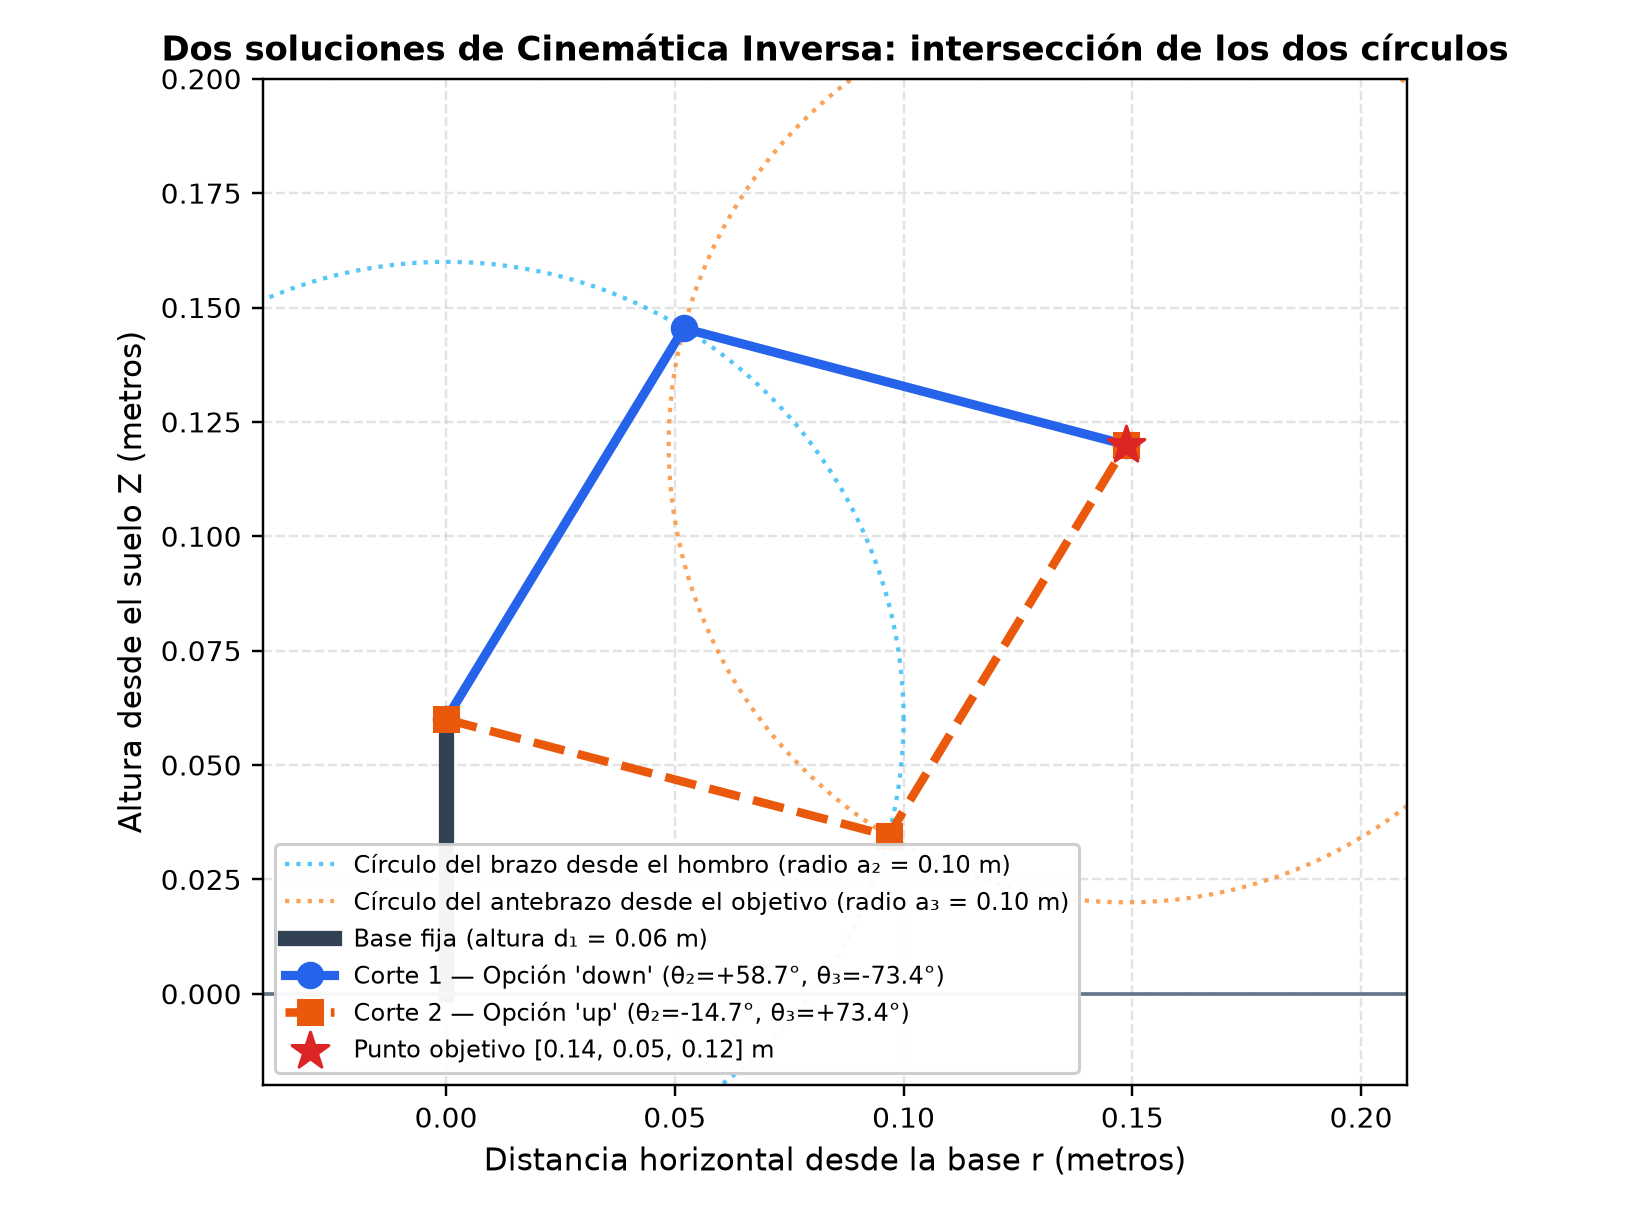
\includegraphics[width=0.78\textwidth]{fig_cinematica_inversa.png}
    \caption{Por qué salen dos soluciones: el círculo del brazo (azul) y el del antebrazo (naranja) se cortan en dos puntos posibles para el codo (\texttt{down} y \texttt{up}).}
    \label{fig:res_proc3}
\end{figure}

En la Figura~\ref{fig:res_proc3} se ve de un vistazo por qué ocurre esto:
\begin{itemize}
    \item El codo tiene que estar a $0.10\text{ m}$ del hombro (círculo azul) y a $0.10\text{ m}$ del objetivo (círculo naranja). Como los dos círculos se cortan en \textbf{dos puntos}, el robot puede elegir ir con el codo por arriba (rama \texttt{down}, azul) o por abajo (rama \texttt{up}, naranja).
    \item \textbf{Prueba con una coordenada válida (Figura~\ref{fig:cap_manual_2}):} Al introducir $[0.14, 0.05, 0.12]\text{ m}$ en la interfaz y pulsar \textit{«Calcular Cinemática Inversa»}, aparece la bola verde en ese punto del espacio 3D y se obtienen los ángulos $[+19.65^\circ, +58.70^\circ, -73.44^\circ]$ lista para ejecutar el movimiento.
    \item \textbf{Prueba con una coordenada inválida (Figura~\ref{fig:cap_manual_3}):} Si pedimos un punto imposible —ya sea porque está demasiado lejos y los dos círculos no se tocan, o porque está demasiado pegado a la base como $[0.030, 0.000, 0.100]\text{ m}$ y obligaría a doblar el codo más de los $90^\circ$ permitidos—, la interfaz avisa en rojo (\textit{«SIN SOLUCIÓN VÁLIDA»}) y bloquea el movimiento para proteger al robot.
\end{itemize}

\begin{figure}[H]
    \centering
    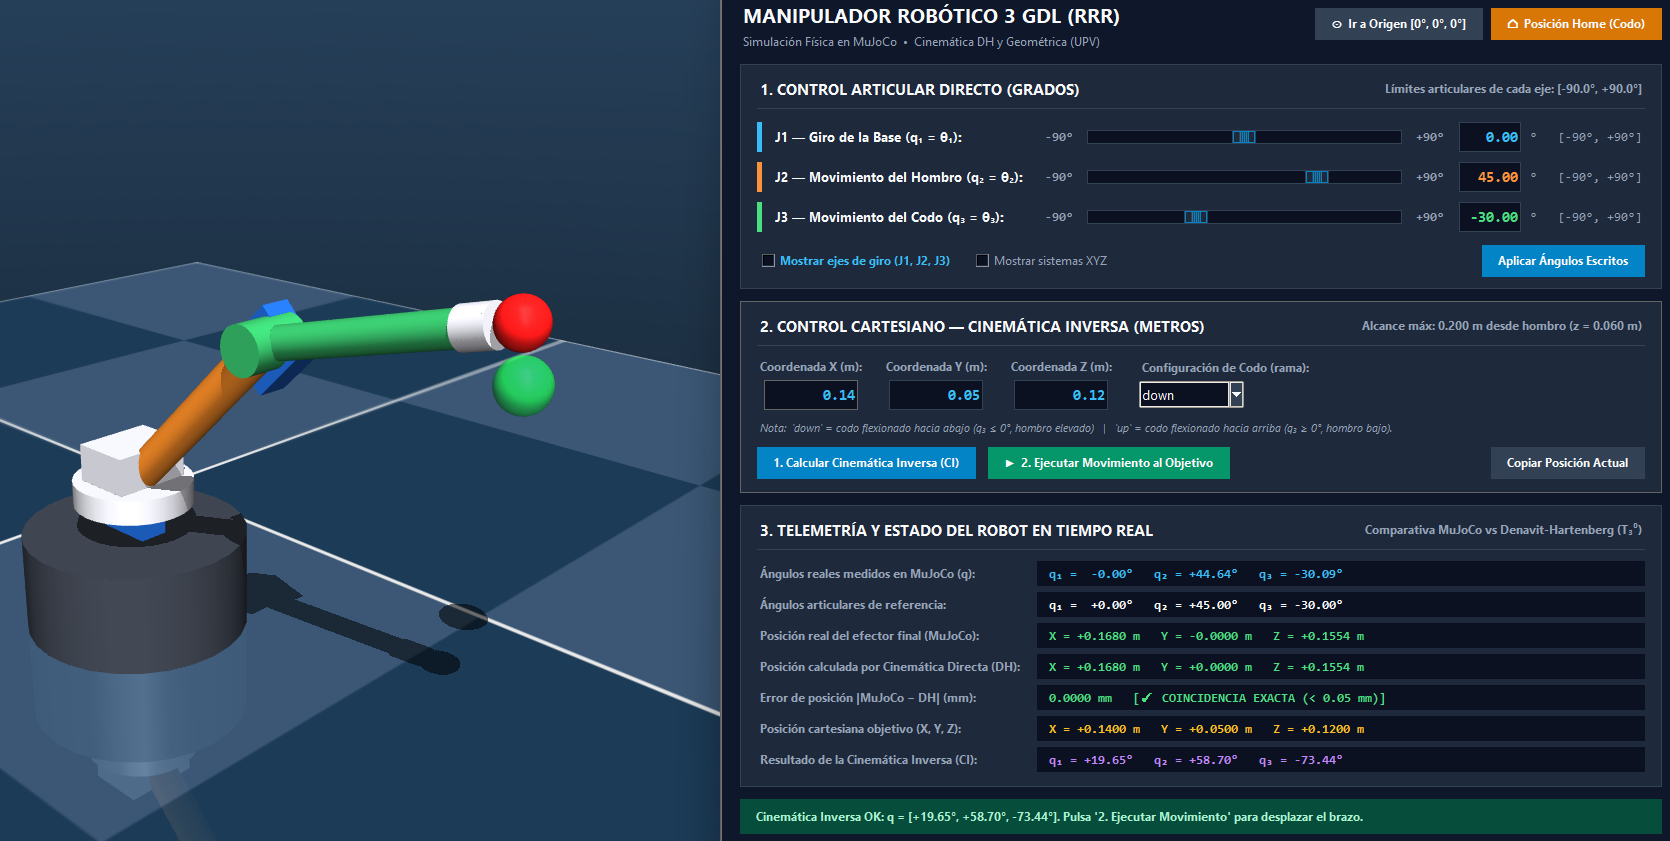
\includegraphics[width=0.92\textwidth]{cordenadaok.png}
    \caption{Cálculo de Cinemática Inversa válido para el objetivo $[0.14, 0.05, 0.12]\text{ m}$ (marcado con la bola verde en el visor 3D).}
    \label{fig:cap_manual_2}
\end{figure}

\begin{figure}[H]
    \centering
    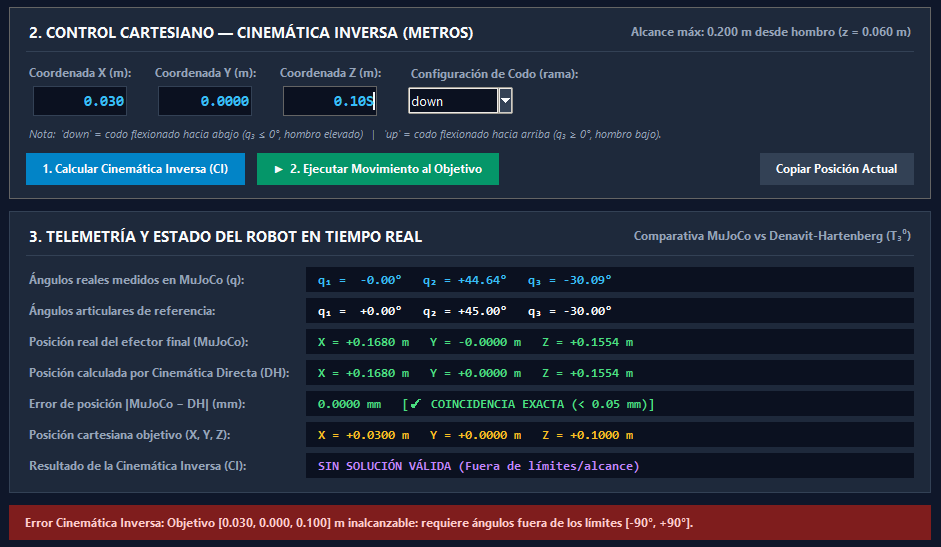
\includegraphics[width=0.88\textwidth]{cordenadaerror.png}
    \caption{Detección de error en la interfaz al introducir una coordenada inalcanzable ($[0.030, 0.000, 0.100]\text{ m}$) que supera los límites de $[-90^\circ, +90^\circ]$.}
    \label{fig:cap_manual_3}
\end{figure}

\textbf{Enlace al vídeo demostrativo:}
En el siguiente enlace se muestra un vídeo corto probando el robot en tiempo real (control por deslizadores, botones de \textit{Home} y \textit{Origen}, visualización de ejes, cinemática inversa y detección de errores):
\begin{itemize}
    \item \textbf{Vídeo del funcionamiento:} \url{https://youtu.be/PONER_AQUI_TU_ENLACE}
\end{itemize}

% ==============================================================================
% 5 CONCLUSIONES
% ==============================================================================
\section{Conclusiones}

\begin{enumerate}
    \item \textbf{Cumplimiento de los objetivos:} Se ha conseguido modelar desde cero el brazo robótico de 3 grados de libertad en MuJoCo y controlarlo mediante su propia interfaz gráfica. Todas las fórmulas de Denavit-Hartenberg y de cinemática inversa geométrica de los apuntes de clase han coincidido exactamente con las medidas del simulador (con un error de $0.0000\text{ mm}$).
    \item \textbf{Comprensión visual de la teoría:} Añadir en la interfaz los botones para alternar entre la postura \textit{Home} (codo flexionado) y el \textit{Origen} matemático ($[0^\circ, 0^\circ, 0^\circ]$ estirado), junto con la visualización de los ejes XYZ y la bola verde objetivo, ha facilitado mucho entender cómo funcionan los sistemas de referencia de Denavit-Hartenberg y las dos soluciones de codo (\texttt{down} y \texttt{up}).
    \item \textbf{Limitaciones del robot actual:} Al tener 3 articulaciones podemos colocar la punta en cualquier coordenada $(X, Y, Z)$ dentro de su alcance, pero no podemos elegir de forma independiente el ángulo con el que se inclina la punta al llegar. Además, como los microservos SG90 tienen un recorrido de $180^\circ$ ($[-90^\circ, +90^\circ]$), el robot solo puede trabajar en la mitad delantera ($X \ge 0$).
    \item \textbf{Trabajos futuros:} Como mejoras futuras se podría añadir una muñeca con 2 o 3 motores más para poder orientar una pinza, programar trayectorias para que la punta se mueva en línea recta usando la matriz Jacobiana, y añadir compensación del peso de la gravedad en el controlador de los motores.
\end{enumerate}

% ==============================================================================
% 6 BIBLIOGRAFÍA
% ==============================================================================
\section{Bibliografía}

\begin{itemize}
    \setlength{\itemsep}{6pt}
    \item[] Bottema, O., y Roth, B. (1979). \textit{Theoretical kinematics}. North-Holland Publishing Company.
    \item[] Corke, P. (2011). \textit{Robotics, vision and control: Fundamental algorithms in MATLAB} (Vol. 73). Springer. \url{https://doi.org/10.1007/978-3-642-20144-8}
    \item[] Denavit, J., y Hartenberg, R. S. (1955). A kinematic notation for lower-pair mechanisms based on matrices. \textit{Journal of Applied Mechanics}, \textit{22}(2), 215--221. \url{https://doi.org/10.1115/1.4011045}
    \item[] Duffy, J. (1980). \textit{Analysis of mechanisms and robot manipulators}. Edward Arnold.
    \item[] Solanes, J. E. (2026). \textit{UD1. Fundamentos del modelado de robots — M11. Cinemática directa e inversa} [Apuntes de clase]. Universitat Politècnica de València (UPV).
    \item[] Todorov, E., Erez, T., y Tassa, Y. (2012). MuJoCo: A physics engine for model-based control. En \textit{2012 IEEE/RSJ International Conference on Intelligent Robots and Systems (IROS)} (pp. 5026--5033). IEEE. \url{https://doi.org/10.1109/IROS.2012.6386109}
\end{itemize}

\end{document}
